
\section{Temporal Analysis}
\label{sec:temporal}

In this section, we study temporal property of VirusTotal malwares. 

\begin{figure}[t!]
\begin{center}
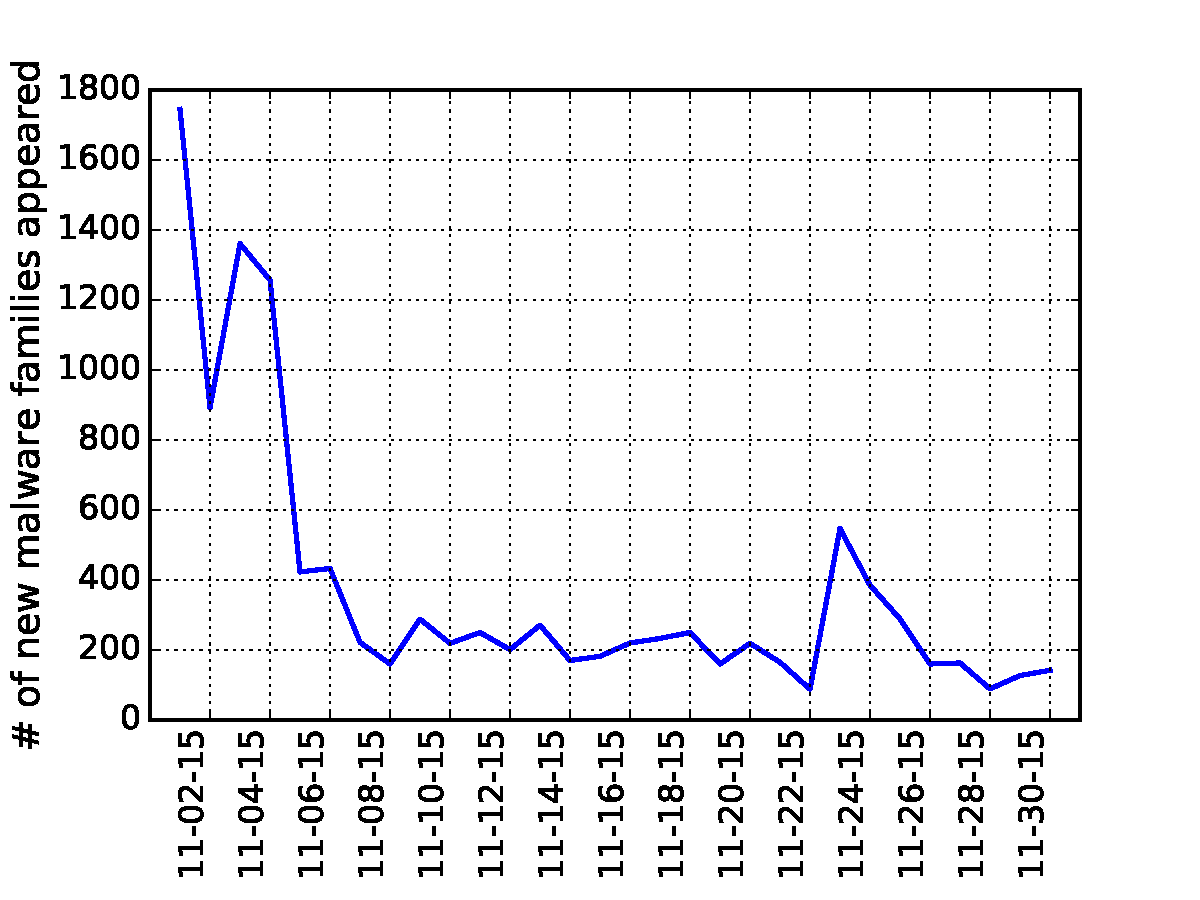
\includegraphics[width=2.5in]{figure/new_family}
\caption{The number of new malware families we observed each day in November of 2015.}
\label{fig:new}
\end{center}
\end{figure}


We first study how many new malware families appear each day. 
Figure~\ref{fig:new} shows the number of new malwares appearing each day in November of 2015. 
We do not have any data before Nov. 1st, 
so there are much more new malware families in the first few days.
After that, the number of new malware families become stable, and falling into the range from 100 to 400. 
In total, there are 11311 malware families. 

{\bf Observation 1:} 
there are 100-400 new malware families appearing each day. 


\begin{figure}[t!]
\begin{center}
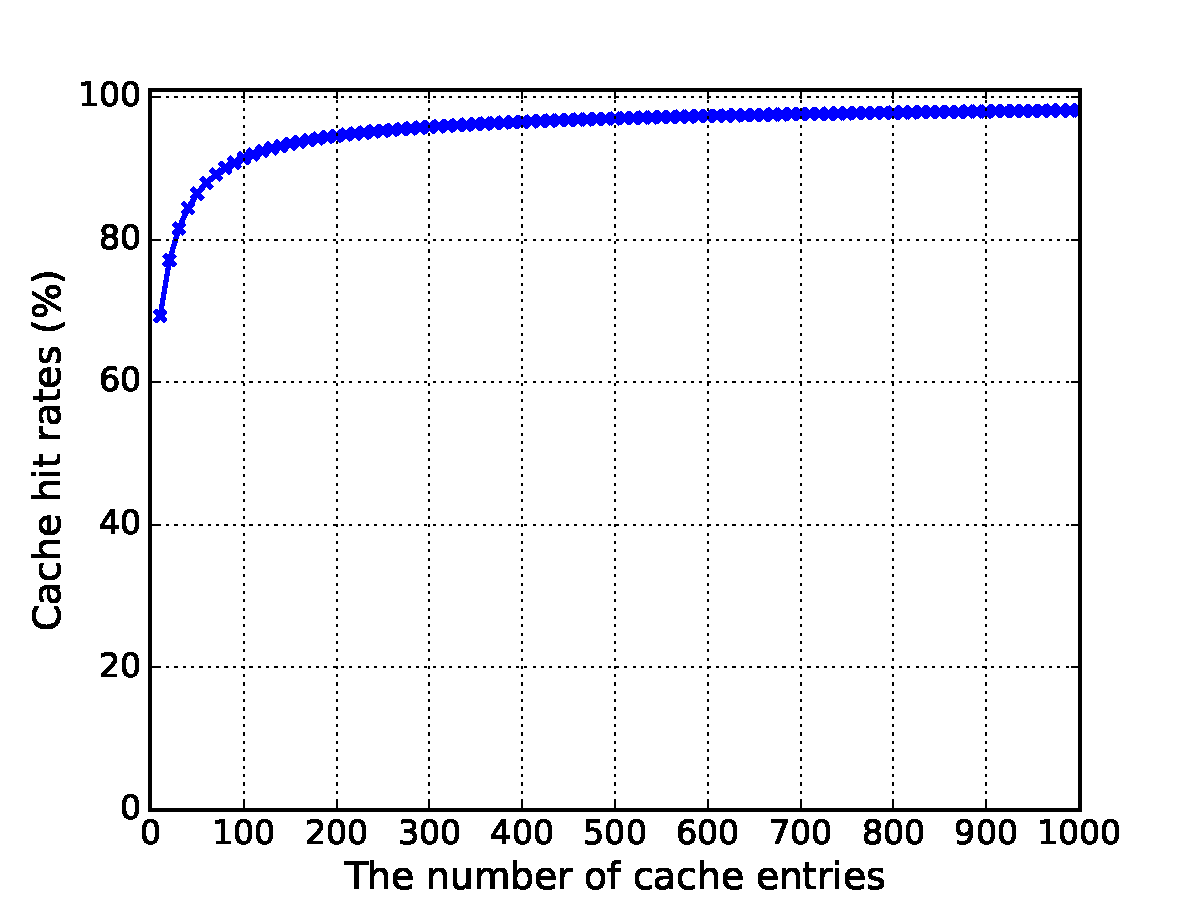
\includegraphics[width=2.5in]{figure/LRU}
\caption{Relation between cache hit rate and cache size.}
\label{fig:cache}
\end{center}
\end{figure}


\begin{figure}[t!]
\begin{center}
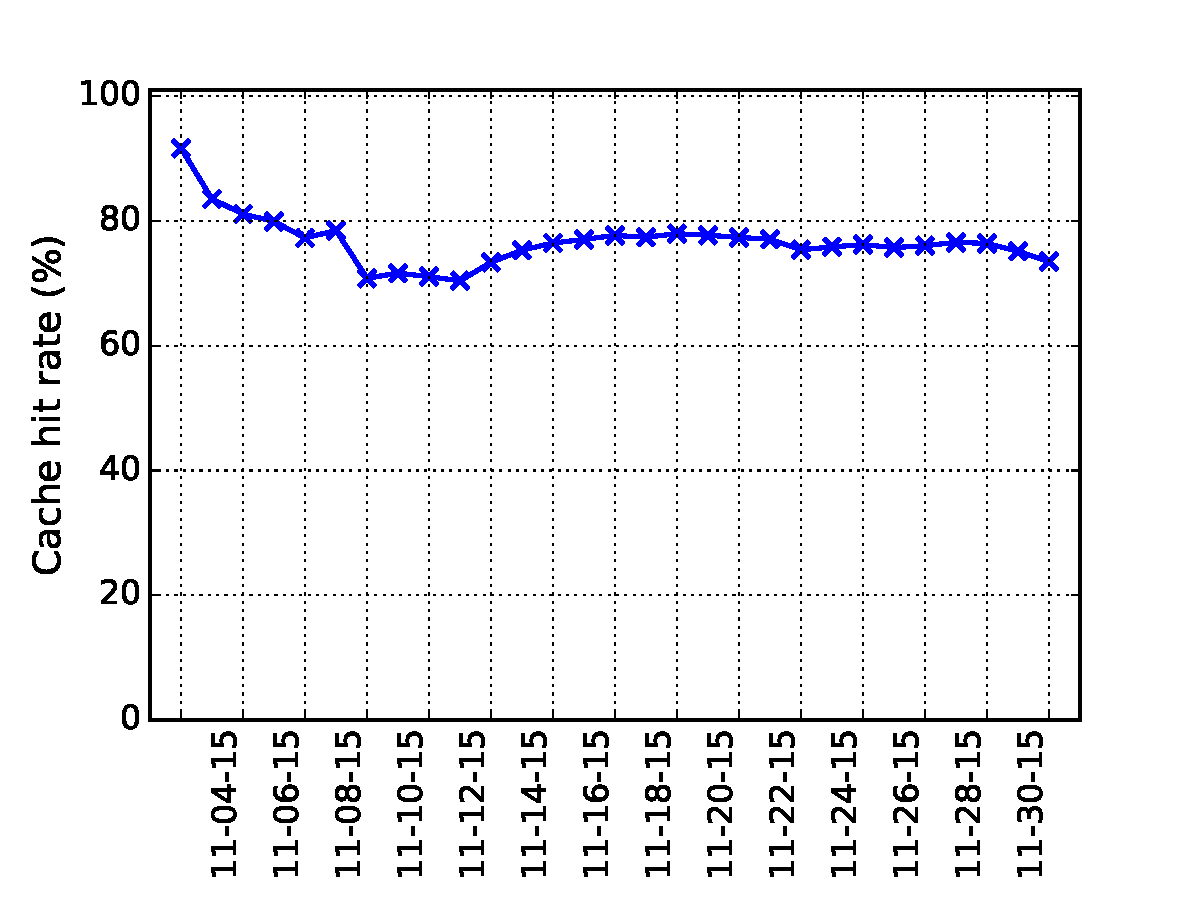
\includegraphics[width=2.5in]{figure/LRU_day}
\caption{Cache hit rate when updating cache content once a day.}
\label{fig:batchcache}
\end{center}
\end{figure}

We then investigate whether there are time locality for malwares.
Specifically, we hypothesize that malwares in the same family would appear in bursts.  
We borrow cache mechanism from system research area to validate our hypothesis. 
Cache was previously used to predict bugs~\cite{predicting}, 
since bugs are introduced not uniformly in time, but in bursts and with strong time locality. 
We view malware submission reports as a stream, 
according to each report’s submission timestamp, and feed the stream into a cache. 
If the cache hit rate is high, 
we can conclude that the appearance of malwares also has time locality. 

There are several notions in cache terminology: 
block size is defined as how many entries would be added into cache or evicted from cache together.
Pre-fetch means loading entries that cache has not encountered yet. 
Replacement policy control how to evict entries from cache, when the cache is full. 
We use the most preliminary cache setting in our evaluation. We fix the block size to be 1, disable pre-fetch, 
and use LRU (least recently used) replacement policy.
Our malware family cache works as follows:  

We start with an empty cache. 
For a new malware submission, if the malware family is already in cache, 
we will move the related cache entry to the front our cache entry list. 
If the new malware family is not in cache, 
we will create a new cache entry, and add it into the front of our cache entry list. 
If our cache is full, we need to evict the entry at the end. 
The cache hit rate is calculated as: 

$$ \mbox{hit rate} = \dfrac{\mbox{\# of hits}}{\mbox{\# of hits + \# of misses}}$$



We conduct two experiments. In the first experiment, 
we explore how cache hit rate changes with the number of cache entries. 
We change cache size from 10 to 1000. As shown in Figure~\ref{fig:cache}, 
the rate rate will grow from 69.29\% to 98.14\%. 
By using more than 80 cache entries, which are less than 1\% of the total number of malware families, the cache hit rate will be above 90\%, 
and by using more than 230 cache entries, which are less than 3\% of the total number of malware families, 
the cache hit rate will be above 95\%. 

In the second experiment, we fix the cache size to 100, 
and we lower the cache content update frequency from once per malware report to once per day, 
that is we keep cache content changed to count cache hit and cache miss each day and update cache content at the end of each day.
Figure~\ref{fig:batchcache} show the cache hit rate each day. 
Most cache hit rate falls in the range from 70\% to 80\%.  


{\bf Observation 2:} 
the appearance of malwares in each family has strong time locality.  

\underline{Discussion.}
Resources to combat malwares are limited. 
Any techniques which could allow antivirus vendors to focus their efforts are great. 
Our cache-based malware prediction technique can predict which malware families would appear in the near future with high precision. 
There are many other cache configurations: 
like different cache block sizes, different pre-fetch mechanisms, 
and different replacement policies. We leave explore the effect of their combinations in the future. 
Currently, we use malware family as prediction granularity. 
In the future, we could try to predict malwares in a finer granularity. 
For example, ssdeep values are also provided in VirusTotal metadata, 
and these values can be used to cluster malwares. 
We could cluster malwares in each family firstly, and then use cluster as prediction granularity. 
